\section{Multicomponent homogeneous systems}

Now we make our first step to increase the complexity of the system under study and let the possible number of components inside the system to increase. Thus, now two type of molecules or atoms can be present inside the material or solution allowing for a much larger phase space to consider. Nevertheless, to still keep the things simple we will assume a \textbf{homogeneous} phase, meaning that the system is composed by different elements in the same phase of matter. Therefore, we will not consider the possibility of having a solid with liquid or gas inside for the moment.
\dfn{Multicomponent homogeneous systems}
{
    We will call a system multicomponent homogeneous if it's composed by different components, molecules or atoms, which are all in the same state of matter: solid, liquid or gass.
}
\noindent
To make an example, the typical system one can think about is an \textbf{alloy}, a terminology used to indicate a solid mixture of two or more chemical elements. The latter is mainly used for metallic solids but can be extended to all materials. An alloy can be homogeneous, in which case is also called a \textbf{solid solution}, where the dominant element is called \textbf{solvent}, and the others \textbf{solutes}. 

To work with these systems we will focus on how the system is composed, looking at how the different elements interact with each other modifying the physical properties of the material. This basically means that a general function of state $f'$ will now depend on the composition of the system in a way that will look like the following
\begin{equation}
    f'(n_1, n_2, n_3, \dots, n_N; T, P) = f'(\vb{n}, T, P),
\end{equation}
Where $n_i$ is the number of mole of the $i$-th component. We can also notice that $f$ has also dependence on the thermodynamical quantities $T$ and $P$ which, nevertheless, are often taken to be constant during experiments. In this context it comes really handy to define some important quantities that will be used extensively during the section.
\dfn{Molar fraction}
{
    Taken the $i$-th component inside a multicomponent system we will define its molar fraction as
    \begin{equation}
        \label{eq:MolarFraction}
        X_i = \frac{n_i}{\sum_j n_j} = \frac{n_i}{n_T}.
    \end{equation}
}
\noindent
Basically we have normalized the number of mole of a component so to work with a simple quantity that allow to know in percentage how much of that component is present inside the material. For example, if $X_i = 1$ that means that only that component is present while $0$ determines its absence. This normalization over $n_T$ is really useful also for the physical quantities, which allow to make them depend on $X_i$ rather than $n_i$. For this reason we will often work with molar functions.
\dfn{Molar function}
{
    Taken a physical quantity $f'$ we will define the molar function deriving from it the value
    \begin{equation}
        \label{eq:MolarFunction}
        f = f'/n_T.
    \end{equation} 
}


At last, it's important to remind to the reader the important difference that exist between \textbf{intensive} and \textbf{extensive} quantities inside a thermodynamic system. It's possible that the reader has already seen this exact definitions in other instances, but it will be useful to rewrite them inside the contest of multicomponent systems. In particular the reader should recall how the difference is usually settled at words as if the quantity is proportional or invariant to variations of the system sizes. Inside our description the size of the system is controlled by the number of moles of the components, therefore we can mathematically state the definition of extensive and intensive in the following way.
\dfn{Extensive quantities}
{
    A thermodynamic quantity $f'$ is sad to be extensive if taken $\lambda > 0$ the following equality holds true
    \begin{equation}
        f'(\lambda\vb{n}, T, P) = \lambda f'(\vb{n}, T, P),
    \end{equation}
    which mathematically means that is a homogeneous function of degree 1.
}
\dfn{Intensive quantities}
{
    A thermodynamic quantity $f'$ is sad to be intensibe if taken $\lambda > 0$ the following equality holds true
    \begin{equation}
        f'(\lambda\vb{n}, T, P) = f'(\vb{n}, T, P).
    \end{equation}
}
\noindent
This ends the series of definitions, now we can start to study the properties of multicomponent systems.



\subsection{Partial molar properties}



Let $f'$ being an extensive thermodynamic quantity that we are interested in studying for our multicomponent system. To approach this problem we may want to have a look to its differential
\begin{equation}
    \dd f' = \grad_{\vb{n}}f' \vdot \dd \vb{n} + \pdv{f'}{T}\dd T + \pdv{f'}{P}\dd P,
\end{equation}
which is usually written by taking $P$ and $T$ constant since in solid state those quantities are easier to be fixed during experiments. In this way we can fully characterize $f'$ in terms of the partial derivatives respect to the number of moles of the components
\begin{align}
    \label{eq:PQdifferential}
    & \overline{f}_i = \eval{\pdv{f'}{n_i}}_{n_{j\neq i}, T, P}, & \dd f' = \sum_i \overline{f}_i\dd n_i.
\end{align}
These derivatives are, therefore, really powerful and will become the main focus of the studies around the physical properties. For this reason we will give them the name of \textbf{partial molar properties} (PMP), and we will define them rigorously as follows.
\dfn{Partial molar properties}
{
    Taken a physical quantity $f'$ the partial molar property related to the $i$-th component of the system is defined to be
    \begin{equation}
        \overline{f}_i = \eval{\pdv{f'}{n_i}}_{n_{j\neq i}, T, P},
    \end{equation}
    which can also be seen as the application of the \textbf{partial molar operator} $\partial/\partial n_i$ to $f'$ itself.
}
\noindent
Thus, we can show effectively how powerful they can be by showing that the knowledge of $\overline{f}_i$ can, not only, shows us how $f'$ changes, but allows also for the function itself to be known without the need of integration. In particular, this result can be obtained in the following way.
\thm{Determination's of physical quantities via PMPs}
{
    Given $f'$ an extensive thermodynamic quantity then the following relation holds true
    \begin{equation}
        \label{eq:PMPproperty1}
        f'(\vb{n}, T, P) = \sum_i \overline{f}_i(\vb{n}, T, P) n_i.
    \end{equation}
}
\pf{Proof}
{
    Since $f'$ is extensive is also a homogeneous function of degree 1, having $f'(\lambda\vb{n}, T, P) = \lambda f'(\vb{n}, T, P)$ of which we can take the derivative respect to $\lambda$ from both sides. The right one simply becomes $f'$, while the right one gets
    \begin{equation}
        \frac{\dd f'}{\dd \lambda}(\lambda\vb{n}, T, P) = \sum_i \frac{\partial f'}{\partial (\lambda n_i)}(\lambda\vb{n}, T, P) \pdv{(\lambda n_i)}{\lambda} = \sum_i \frac{\partial f'}{\partial (\lambda n_i)}(\lambda\vb{n}, T, P) n_i.
    \end{equation}
    So, by setting the two parts equal to each others we have
    \begin{equation}
        \sum_i \frac{\partial f'}{\partial(\lambda n_i)}(\lambda\vb{n}, T, P) n_i = f'(\vb{n}, T, P),
    \end{equation}
    where $\lambda = 1$ gives the wanted relation.
}

Here we can start to see how the quantities expressed in molar terms can be powerful, even if someone may ask if we are not simply complicating things by the need now of determining $N$ values of $\overline{f}_i$ instead of simply $f'$. The reason for it is that some interesting properties can be found out for the PMPs that are general and will allow for their computations.
\cor{PMPs are intensive quantities}
{
    Taken an extensive physical quantity $f'$ its PMPs are all intensive ones.
}
\pf{Proof}
{
    We can start from \eqref{eq:PMPproperty1} and from it apply the transformation $\vb{n} \to \lambda \vb{n}$, we will have
    \begin{equation}
        f'(\lambda\vb{n}, T, P) = \lambda\sum_i \overline{f}_i(\lambda\vb{n}, T, P)n_i = \lambda\sum_i \overline{f}_i(\vb{n}, T, P) n_i.
    \end{equation}
    For the two expressions to be equal we need that $\overline{f}_i(\lambda\vb{n}, T, P) = \overline{f}_i(\vb{n}, T, P)$ making $\overline{f}_i$ intensive quantities.
}
\noindent
This is interesting under a physical point of view since we can evaluate $\overline{f}_i$ in systems without caring about the sizes and still having exact values for every possible compositions. Also, this means that we can imagine at $\overline{f}_i$ like \textbf{properties of the single components} of the systems, so that do not depend on their quantities but only on their atomistic properties. Along with that, we can also see how every one of them influences the others since also a relation between the differentials can be found out.
\cor{Gibbs-Duhem equation}
{
    Taken an extensive physical quantity $f'$ the differentials of the PMPs relates using this equation
    \begin{equation}
        \sum_i n_i \dd \overline{f}_i = 0.
    \end{equation}
}
\pf{Proof}
{
    Using \eqref{eq:PMPproperty1} we can write down the differential of $f'$ as follows
    \begin{equation}
        \dd f' = \sum_i \overline{f}_i \dd n_i + \sum_i n_i \dd \overline{f}_i = \dd f' + \sum_i n_i \dd \overline{f}_i,
    \end{equation}
    where \eqref{eq:PQdifferential} was used to rewrite the differential. Then, by rearranging, the wanted relation is obtained.
}

As a last remark we can also show that these molar quantities retains some of the same properties of the normal thermodynamical quantities. In particular, every thermodynamic potential posses a PMP counterpart defined in the same way as the normal one. For example, the Gibbs free energy $G' = H' - TS'$ can be written, by appling the partial molar operator
\begin{equation}
    \overline{G}_i = \overline{H}_i - T \overline{S}_i,
\end{equation}
which tells that all the knwon thermodynamic relations remains true, like
\begin{align}
    &\overline{S}_i = -\eval{\pdv{\overline{G}_i}{T}}_{n_k, P}, &\overline{V}_i = \eval{\pdv{\overline{G}_i}{P}}_{n_k, T}.
\end{align}
Along with that, also the Maxwell relations or the differentials remains unchanged we only need to substitute the PMP's version of the quantity present in the normal relation. The only change between the normal and PMP cases worth noticing is the value of $\overline{G}_i$, which we have already seen that becomes $\mu$ inside a unary system and here things doesn't change since
\begin{align}
    & \dd G' = - S'\dd T + V'\dd P + \sum_i \mu_i \dd n_i, & \mu_i = \eval{\pdv{G'}{n_i}}_{n_{k\neq i}, P, T} = \overline{G}_i.
\end{align}
Thus, everything related to the Gibbs free energy will become a relation using the chemical potential\footnote{Keep in mind that this happens only because we have decied to work at constant $P$ and $T$ for experimental simplicity, in a general situation we may keep constant other quantities and then $G$ will no more be the potential of choice while another may become the right one whose PMP gives $\mu$.}.

\ex{}
{
    With these results we are able to already study some simple systems in an analytic form. For example, let's take a two component system and study the behavior of a molar function $f(X_1, X_2; T, P)$. Since we are using the molar version of $f'$ we can also rewrite it differential that becomes
    \begin{equation}
        \dd f  = \overline{f}_1 \dd X_1 + \overline{f}_2 \dd X_2,
    \end{equation}
    but we also know that $X_1 + X_2 = 1$ leading to $\dd X_1 = -\dd X_2$. Thus, we can find out the derivative of $f$ as
    \begin{equation}
        \dv{f}{X_2} = \overline{f}_2 - \overline{f}_1,
    \end{equation}
    we only need to write down the two quantities.  The idea is that we know from \eqref{eq:PMPproperty1} that $f = \overline{f}_1 X_1 + \overline{f}_2 X_2$, so by substituting $X_1 = 1 - X_2$ we have
    \begin{equation}
        \overline{f}_1 = \frac{f - \overline{f}_2X_2}{1 - X_2}.
    \end{equation}
    Thus, by inserting it inside the derivative of $f$ found previously we obtain a general simple relation for the physical quantity
    \begin{equation}
        \label{eq:BynaryPMP}
        f = \overline{f}_1 + (X_2 - 1)\dv{f}{X_2},
    \end{equation}
    same computations can be done for $X_1$ leading to the same results but with inverted subscripts. Basically, using really simple considerations we were able to obtain a general result for $f$ that allow us to study the system simply, but most importantly gives us a geometric way of evaluating the PMPs. In fact the \eqref{eq:BynaryPMP} can be rewritten in terms of $\overline{f}_1$ and taken a fixed point $X_2^0$ one can see how it describes a line coming from the point to the intercept with the y-axis as is illustrated in \figref{fig:PMPs}.
}

\begin{figure}[t]
    \centering
    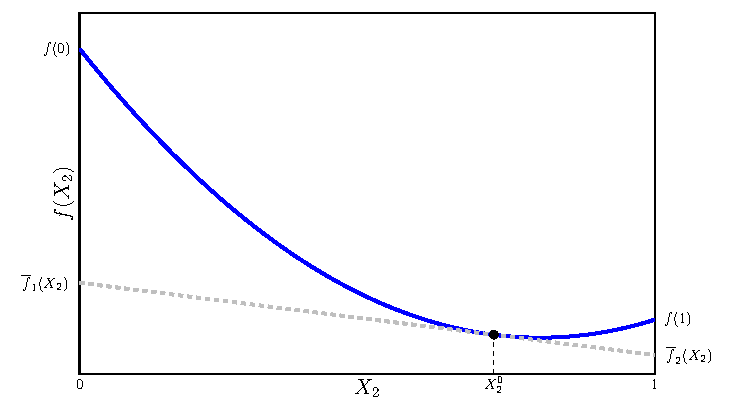
\includegraphics[width=0.8\linewidth]{Immagini/PMPs.pdf}
    \caption{
        Illustration of the graphical method to compute the PMPs of a binary system in the case of a simple physical quantity. It's possible to see how the method basically select one point $X_2^0$ and then draw the tangent to $f$ in that point finding the PMPs as the intercepts with the $X_2 = 0$ and $X_2 = 1$ axis.
    }
    \label{fig:PMPs}
\end{figure}

\nt
{
    The result obtained not only showed us the power of PMPs but also that they are not independent of the material composition. In fact the values of $\overline{f}_i$ changed based on the point $X_2^0$ taken. The only situation where they are independent is when $f$ is linear in $X_i$, which is obvious since the PMPs are the derivative of $f$ respect to $X_i$ and so if it's linear the $X_i$ dependence go away.
}

\subsection{Mixing process}

The next step is studying how the physical quantities changes due to the mixing of the various components. Thus, we can imagine to gradually insert an element inside the system and has the molar fractions changes look at how a certain $f$ changes, and this can be written as
\begin{equation}
    \label{eq:MixingQuantity}
    \Delta f_{mix} = \sum_i \overline{f}_i X_i - \sum_i f_i^\circ  X_i = \sum_i \Delta \overline{f}_i X_i,
\end{equation}
where $f_i^\circ$ represent $\overline{f}_i$ evaluated in the point where $X_i = 0$. This has shown how the variation of the physical quantities can be directly expressed in terms of the PMPs, and in particular of what we will call the \textbf{PMPs of mixing} $\Delta \overline{f}_i$. For this reason we are interested in look also at the properties of these quantities, in particular it's easy to see that a version of Gibbs-Duhem equation can be written for them.
\thm{Gibbs-Duhem equation for mixing}
{
    Taken an extensive physical quantity $f'$ the differentials of the PMPs of mixing relates using this equation
    \begin{equation}
        \label{eq:GDmixing}
        \sum_i\dd (\Delta \overline{f}_i) X_i = 0.
    \end{equation}
}
\pf{Proof}
{
    We start by evaluating the differential of \eqref{eq:MixingQuantity} in order to have, by using Einstein notation
    \begin{equation}
        \dd (\Delta f_{mix}) = \dd \overline{f}_i X_i + \overline{f}_i\dd X_i - \dd f_i^\circ - f_i^\circ \dd X_i = \Delta \overline{f}_i \dd X_i.
    \end{equation}
    Where we can see how $f_i^\circ$ being constant has null differential, while the normal G-D equation lead to $\dd \overline{f}_i X_i = 0$ having so
    \begin{equation}
        \label{eq:ProfG-Dmix1}
        \dd (\Delta f_{mix}) = \Delta \overline{f}_i \dd X_i.
    \end{equation}
    Nevertheless, we can also write down the differential of the mixing quantity by differentiating the last equality in \eqref{eq:MixingQuantity} and having
    \begin{equation}
        \label{eq:ProfG-Dmix2}
        \dd (\Delta f_{mix}) = \dd (\Delta \overline{f}_i) X_i + \Delta \overline{f}_i \dd X_i,
    \end{equation}
    so to have equality between \eqref{eq:ProfG-Dmix1} and \eqref{eq:ProfG-Dmix2} the wanted relation needs to hold true.
}

\ex{}
{
    Also in this case we can look at an exercise to compute the PMPs of mixing given in a binary system once the enthalpy of mixing is given as $\Delta H_{mix} = a X_1X_2$. To do it we can use the same result obtained in the previous example and start with
    \begin{equation}
        \Delta \overline{H}_1 = \Delta H_{mix} - \dv{(\Delta H_{mix})}{X_2} X_2,
    \end{equation}
    and using $X_1 = 1 - X_2$ we can arrive to the final result
    \begin{align}
        &\Delta \overline{H}_1 = a X_2^2, & \Delta \overline{H}_2 = a X_1^2.
    \end{align}
    Where for $\Delta \overline{H}_2$ we used the same exact approach described here, even if it's possible to evaluate it also by the value of $\Delta \overline{H}_1$. In fact, we can use the G-D equation to write down $\dd \Delta \overline{H}_2 = - X_1/X_2 \dd \Delta \overline{H}_1$ where, by using $X_2 = 1 - X_1$ and integrating we have
    \begin{equation}
        \Delta \overline{H}_1 = \int_0^{X_1} \frac{X_1'}{(X_1' - 1)} 2a(X_1' - 1) \dd X_1' = a X_1^2.
    \end{equation}
}

\subsection{Activity and solutions}

The activity $a_i$ of a system is a variable strictly related to the mixing phenomena described previously. In particular, we are going to define it mathematically in the following way.
\dfn{Activity}
{
    The activity of a solution $a_i$ evaluate the variation of free energy on the $i$-th component due to a mixing phenomena as
    \begin{equation}
        \label{eq:defActivity}
        \Delta\mu_i = \mu_i - \mu_i^\circ = RT\ln a_i.
    \end{equation}
}
\noindent
In this simple definition one can understand easily that for an \textbf{ideal solution} the activity will simply be $a_i = X_i$, also called \textbf{Raoult's law}. This result will also lead to other interesting forms for certain quantities in the idea case as
\begin{align}
    &\Delta \overline{S}_i = - \eval{\pdv{\Delta\mu_i}{T}}_{n_k, P} = -R\ln X_i, &\Delta \overline{V}_i = \eval{\pdv{\Delta\mu_i}{P}}_{n_k, T} = 0.
\end{align}
We can so insert them inside the definition of the mixing thermodynamic potential and obtain some other results as
\begin{equation}
    \Delta H_{mix} = 0, \hspace{1.5cm}\Delta G_{mix} = RT\sum_i X_i\ln X_i, \hspace{1.5cm} \Delta S_{mix} = -R\sum_i X_i\ln X_i.
\end{equation}
Where we can recall for $\Delta S_{mix}$ a form totally analogous to the \textbf{Shannon entropy}.

Nevertheless, all of this was only an ideal case, we can also try to study the real one by inserting the non ideality inside a \textbf{activity coefficient} $\gamma_i$ defined as
\begin{equation}
    a_i = \gamma_i X_i.
\end{equation}
If we insert this definition inside \eqref{eq:defActivity} we will have that two part of the variation appears
\begin{equation}
    \Delta\mu_i = RT\ln X_i + RT \ln \gamma_i = \Delta\mu_i^{id} + \Delta\mu_i^{xs},
\end{equation}
where $\Delta\mu_i^{xs}$ is what changes from ideality. We can so use these coefficients to study the evolution of the chemical potential inside our system also because another G-D equation can be written for them.
\cor{Gibbs-Duhem equation for activity coefficient}
{
    Taken an extensive physical quantity $f'$ the differentials of the reactivity coefficients relates using this equation
    \begin{equation}
        \sum_i\dd (\ln \gamma_i) X_i = 0.
    \end{equation}
}
\pf{Proof}
{
    To demonstrate it one can take the differentials of $\Delta\mu_i$ and then use the relation \eqref{eq:GDmixing} to obtain the wanted one, all the tedious mathematical details are left to the reader.
}
\noindent
Using this relation we can have a lot of information on the mixing properties of the material, for example is possible to demonstrate the \textbf{Henry's law} for dilute solutions
\begin{equation}
    \lim_{X_i \to 0} a_i = \gamma_i^\circ X_i.
\end{equation}
Where we have only seen the result in the context of binary systems, but I believe that is kind of general, meaning that in the case of really low solute, $X_2 \to 0$, the solvent, $X_1\to 1$ shows ideal behavior with $\gamma_1 \to 1$, as shown in \figref{fig:HenryLaw}.

\begin{figure}[t]
    \centering
    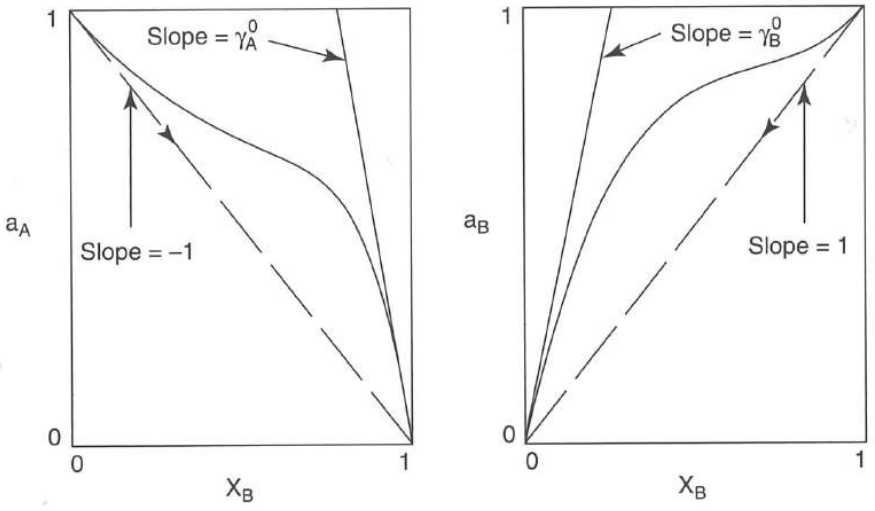
\includegraphics[width=0.6\linewidth]{Immagini/HenryLaw.png}
    \caption{
        Illustration of the activity inside a binary system composed by the phases $a$ and $b$, showing the expected behaviors of ideality in the diluted case. 
    }
    \label{fig:HenryLaw}
\end{figure}

Another type of situation that we are interested in is a particular type of systems called \textbf{regular solutions} that are defined in the following way.
\dfn{Regular solutions}
{
    A solution is called regular if the following two conditions are respected:
    \begin{enumerate}
        \item The entropy of mixing is the same as for ideal solutions
            \begin{equation}
                \Delta S_{mix} = -RX_i \ln X_i.
            \end{equation}
        \item The enthalpy of mixing is different from zero
            \begin{equation}
                \Delta H_{mix} = \Delta H_{mix}^[xs] \neq 0.
            \end{equation}
    \end{enumerate}
}
\noindent
Some things can already be sad for such systems, in fact we can easily say that the excess entropy of mixing, $\Delta S_{mix}^{xs}$, is necessary zero. Meaning that also the following is true
\begin{equation}
    \pdv{\Delta H^{xs}_{mix}}{T} = \pdv{\Delta G_{mix}^{xs} - T\Delta S_{mix}^{xs}}{T} = \pdv{\Delta G_{mix}^{xs}}{T} = -\Delta S_{mix}^{xs} = 0,
\end{equation}
so the enthalpy of the solution shall not depend on the temperature. Thus, this also implies that the variation from ideality is given by the enthalpy change having
\begin{align}
    \Delta\mu_i^{xs} = \Delta \overline{H}_i,
\end{align}
and recalling $\Delta\mu_i^{xs} = RT\ln\gamma_i$ we can find out a general relation for the reaction coefficients
\begin{equation}
    \label{eq:reactionCoeffRS}
    \gamma_i = \exp\left( \frac{\Delta \overline{H}_i}{RT} \right),
\end{equation}
that can be really useful in some situations.

\ex{}
{
    \label{ex:SimpleEnthalpy}
    To make an example of where the relation \eqref{eq:reactionCoeffRS} can be really useful. Basically the simplest model possible for a regular solution posses as excess enthalpy the quantity $H_{mix}^{xs} = aX_1X_2$, that we have already studied, and we know have $\Delta \overline{H}_i = aX_i^2$, so
    \begin{equation}
        \gamma_i = \exp\left( \frac{ aX_i^2}{RT} \right).
    \end{equation}
    This result also shows how $\lim_{X_i\to 1} \gamma_i$ does not depend on $X_i$ so that for the dilute solution the Henry's law holds. Using the form of $\gamma_i$ the values of $\Delta S_{mix}$ and $\Delta G_{mix}$ can be obtained as shown in \figref{fig:SimpleRegularSolution}.
}

\begin{figure}[t]
    \centering
    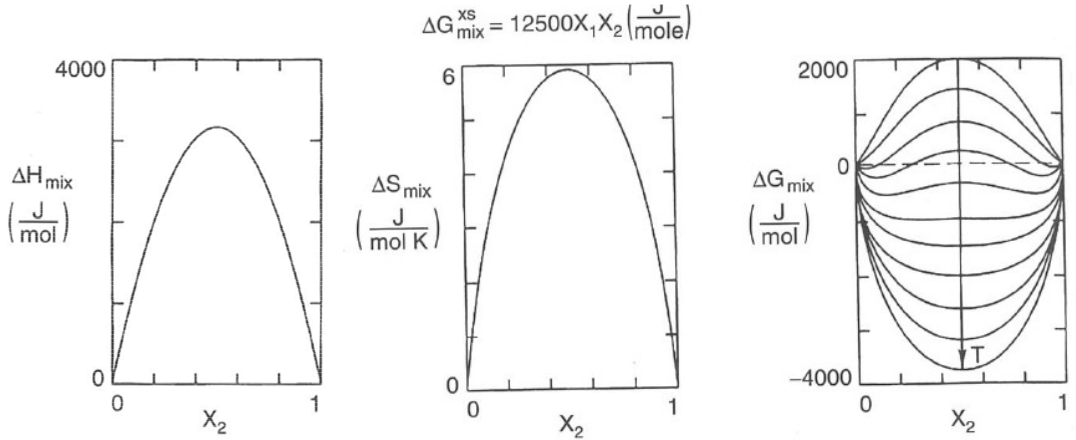
\includegraphics[width=\textwidth]{Immagini/SimpleRegularSolution.png}
    \caption{
        Computed values of mixing properties for the simple system given by the mixing enthalpy $aX_1X_2$. It's possible to see how only the mixing free energy has a temperature dependence, and it's interesting that for some values of $T$ a curve with two global minima is obtained. 
    }
    \label{fig:SimpleRegularSolution}
\end{figure}

\nt
{
    It's interesting to see how also inside the simple system defined in the Ex. (\ref{ex:SimpleEnthalpy}) for certain values of $T$ the solution $\Delta G_{mix}$ posses two global minima. This means that the system doesn't know on which minima should go, basically becomes a frustrated system which minimize the energy not only going into one of the minima, but different parts of the system can go in different minima generating different phases. This is the way in which heterogeneous systems originates in nature. 
}

\subsection{Atomistic model for binary systems}

So far we have focused mainly on the general description of thermodynamic properties inside a general system. Now the aim is to look deeper into a specific system trying to create a microscopic atomistic model that describes the behavior of binary systems. Basically we will imagine to work with a system composed of two types of elements $A$ and $B$ that can occupy two different lattice sites $\alpha$ and $\beta$ on the unit cell of the material. The goal is to describe how the atoms position themselves inside the lattice on average, and in general the possible scenarios are the three depicted inside \figref{fig:SistemiBiatomici}.
\begin{figure}[t]
    \centering
    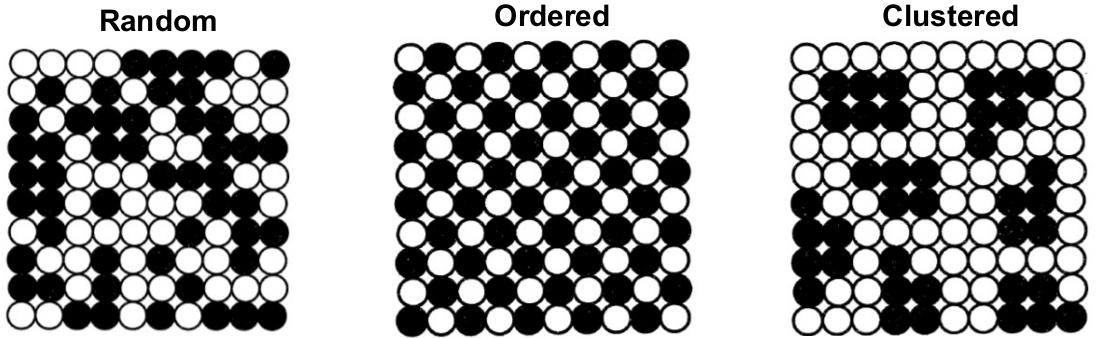
\includegraphics[width=\linewidth]{Immagini/SistemiBiatomici.png}
    \caption{
        Illustration of the three possible type of distributions of the atoms inside a binary system, with the possibility of randomly placed atoms, ordered structure creating a known lattice and clustered systems.
    }
    \label{fig:SistemiBiatomici}
\end{figure}

To study which type of structure will be the one found out inside a material we will use a \textbf{quasi-chemical model}, meaning that we will focus on the bonds that can be generated between nearest neighbors atoms, whose number if given by the coordination one $Z$, and their strength. To do so we will need to consider three types of bonds and the energy gain that they bring to the system: $E_{AA}$ for $A-A$ bonds, $E_{BB}$ for $B-B$ bonds and $E_{AB}$ for $A-B$ bonds. Before entering the computations will be useful to define two \textbf{orders parameters} that will simply the treatment of the system
\begin{align}
    \label{eq:orderParameters}
    &X_i = \frac{1}{2}\left( X_i^\alpha + X_i^\beta \right), &\eta = \frac{1}{2}\left( X_B^\alpha - X_B^\beta \right),
\end{align}
where $X_i^j$ describe the molar fraction of atoms $i$ inside the site $j$. It's important to notice that both the parameters are limited, in the sense that from the properties of molar fractions we can find out how
\begin{align}
    &0 \le X_i \le 1, &-\frac{1}{2} \le \eta \le \frac{1}{2}.
\end{align}
Also, using some further mathematical consideration one can find out how $\eta \le \min(X_B, X_A)$. In physical terms, one can understand how the two quantities are intrinsically different since inside a closed system the total number of atoms $N$ is conserved along with also the two numbers of $A$ and $B$ atoms. This means that the value of $X_A$ and $X_B$ are \textbf{conserved quantities} inside closed systems, while $\eta$ can still change being dependent also on the order with which the atoms position themselves inside the lattice. In particular, one can easily understand that if we call $P(B, \alpha)$ and $P(B, \beta)$ the probabilities of having a $B$ atom in site $\alpha$ or $\beta$, and we assume $N_{B}^i$ to be averages we can write $X_B^j = N_B^j/N = P(B, j)$ having
\begin{equation}
    \eta = \frac{1}{2}\left( X_B^\alpha - X_B^\beta \right) = \frac{1}{2}\left[ P(B, \alpha) - P(B. \beta) \right].
\end{equation}
Showing how $\eta$ is zero only if I have the same probability of having $B$ on one site or the other, therefore a \textbf{random lattice}, while will be maxed out if I'm sure that $B$ atoms are on a specific site generating the maximum order inside the system, \textbf{ordered lattice}.
\nt
{
    It's interesting to point out that even if $\eta$ increasing means an increase in order that doesn't mean that there is also an increase in the symmetry. In fact, increasing order could mean also a decrease in the symmetry. For example in the case of a bcc binary system, if a random lattice is present on average I have same probability of having A or B atoms on the diagonal, creating the pattern $A/B-A/B-A/B-etc$. If, instead, Order comes into play I have a structure of the type $A-B-A-B-etc$ which has less symmetry.
}

Using these informations we can simply write down forms to describe the average number of different types of bonds present inside the material by using an equation of the type
\begin{equation}
    N_{ij} = \frac{\text{number of bonds present}}{2} \times P(i, \alpha) P(j, \beta),
\end{equation}
where the division by $2$ is due to the fact that we don't want to count the same bond twice. In this way we can directly write down general forms for the number of bonds in the following way
\begin{align}
    \label{eq:NumberOfAtoms}
    &N_{AA} = \frac{NZ}{2}X_A^\alpha X_A^\beta = \frac{NZ}{2}\left[ (1 - X_B)^2 - \eta^2 \right],\\
    &N_{BB} = \frac{NZ}{2}X_B^\alpha X_B^\beta = \frac{NZ}{2}\left[ X_B^2 - \eta^2 \right],\\
    &N_{AB} = \frac{NZ}{2}\left( X_A^\alpha X_B^\beta + X_B^\alpha X_A^\beta\right) = \frac{NZ}{2}\left( X_AX_B + \eta^2 \right).
\end{align}
We can now set the number of atoms inside the system to the Avogadro number, to have all quantities referring to one mole, and then compute the energy of the system coming from the bonds
\begin{equation}
    U = N_{AA} E_{AA} + N_{BB} E_{BB} + N_{AB} E_{AB}.
\end{equation}
Still our main interesting is in how the two atoms mix inside the system, so we can write the mixing energy by using as a starting point the case where the two types of atom were separated in different systems having
\begin{equation}
    \Delta U_{mix} = U - \frac{N_A Z}{2}E_{AA} - \frac{N_B Z}{2}E_{BB}.
\end{equation}
By using the definitions in \eqref{eq:NumberOfAtoms} and some algebra we can rewrite the mixing energy in a close form depending on the order parameters as
\begin{equation}
    \Delta U_{mix} = NZ\left( X_AX_B + \eta^2 \right)\left[ E_{AB} - \frac{1}{2}\left(E_{AA} + E_{BB}\right) \right].
\end{equation}